\chapter{Introduction}
\label{sec:intro}

\begin{figure}
  \begin{subfigure}{0.5\textwidth}
    \includegraphics[width=\textwidth]{figures/experiments/experiment-setup-no-funnel}
    \caption{The airplane is deviating from the nominal trajectory due to the
      cross-wind.}
  \end{subfigure}%
  \;
  \begin{subfigure}{0.5\textwidth}
    \includegraphics[width=\textwidth]{figures/experiments/experiment-setup-funnel}
    \caption{The reachable set given the cross-wind pictured.}
  \end{subfigure}
  \caption{Not taking uncertainty into account can lead to collisions when the
    actual trajectory diverges from the nominal one.}
  \label{fig:motion-planning-uncertainty}
\end{figure}

Planning with uncertainty is necessary in order for an algorithm to move out of
the lab and into the real world as in reality there are always uncertainty in
planning. Knowledge of position, the environment and the dynamics of the system
are all uncertain to some degree. Sensory noise, tuning and readings may be off.
Limited precision, and accidents may hinder the measurements and leave them with
an error term. Thus in order for a planner to guarantee safe traversal through a
real world environment, a motion planner needs to handle uncertainties. A
pictorial representation of a planner with and without robustness guarantees is
shown in \cref{fig:motion-planning-uncertainty}. Over the last couple of decades
a lot of research has gone into handling uncertainty in planning, an overview of
which can be found in \cref{chp:survey-of-papers}.

\begin{figure}
  \centering
  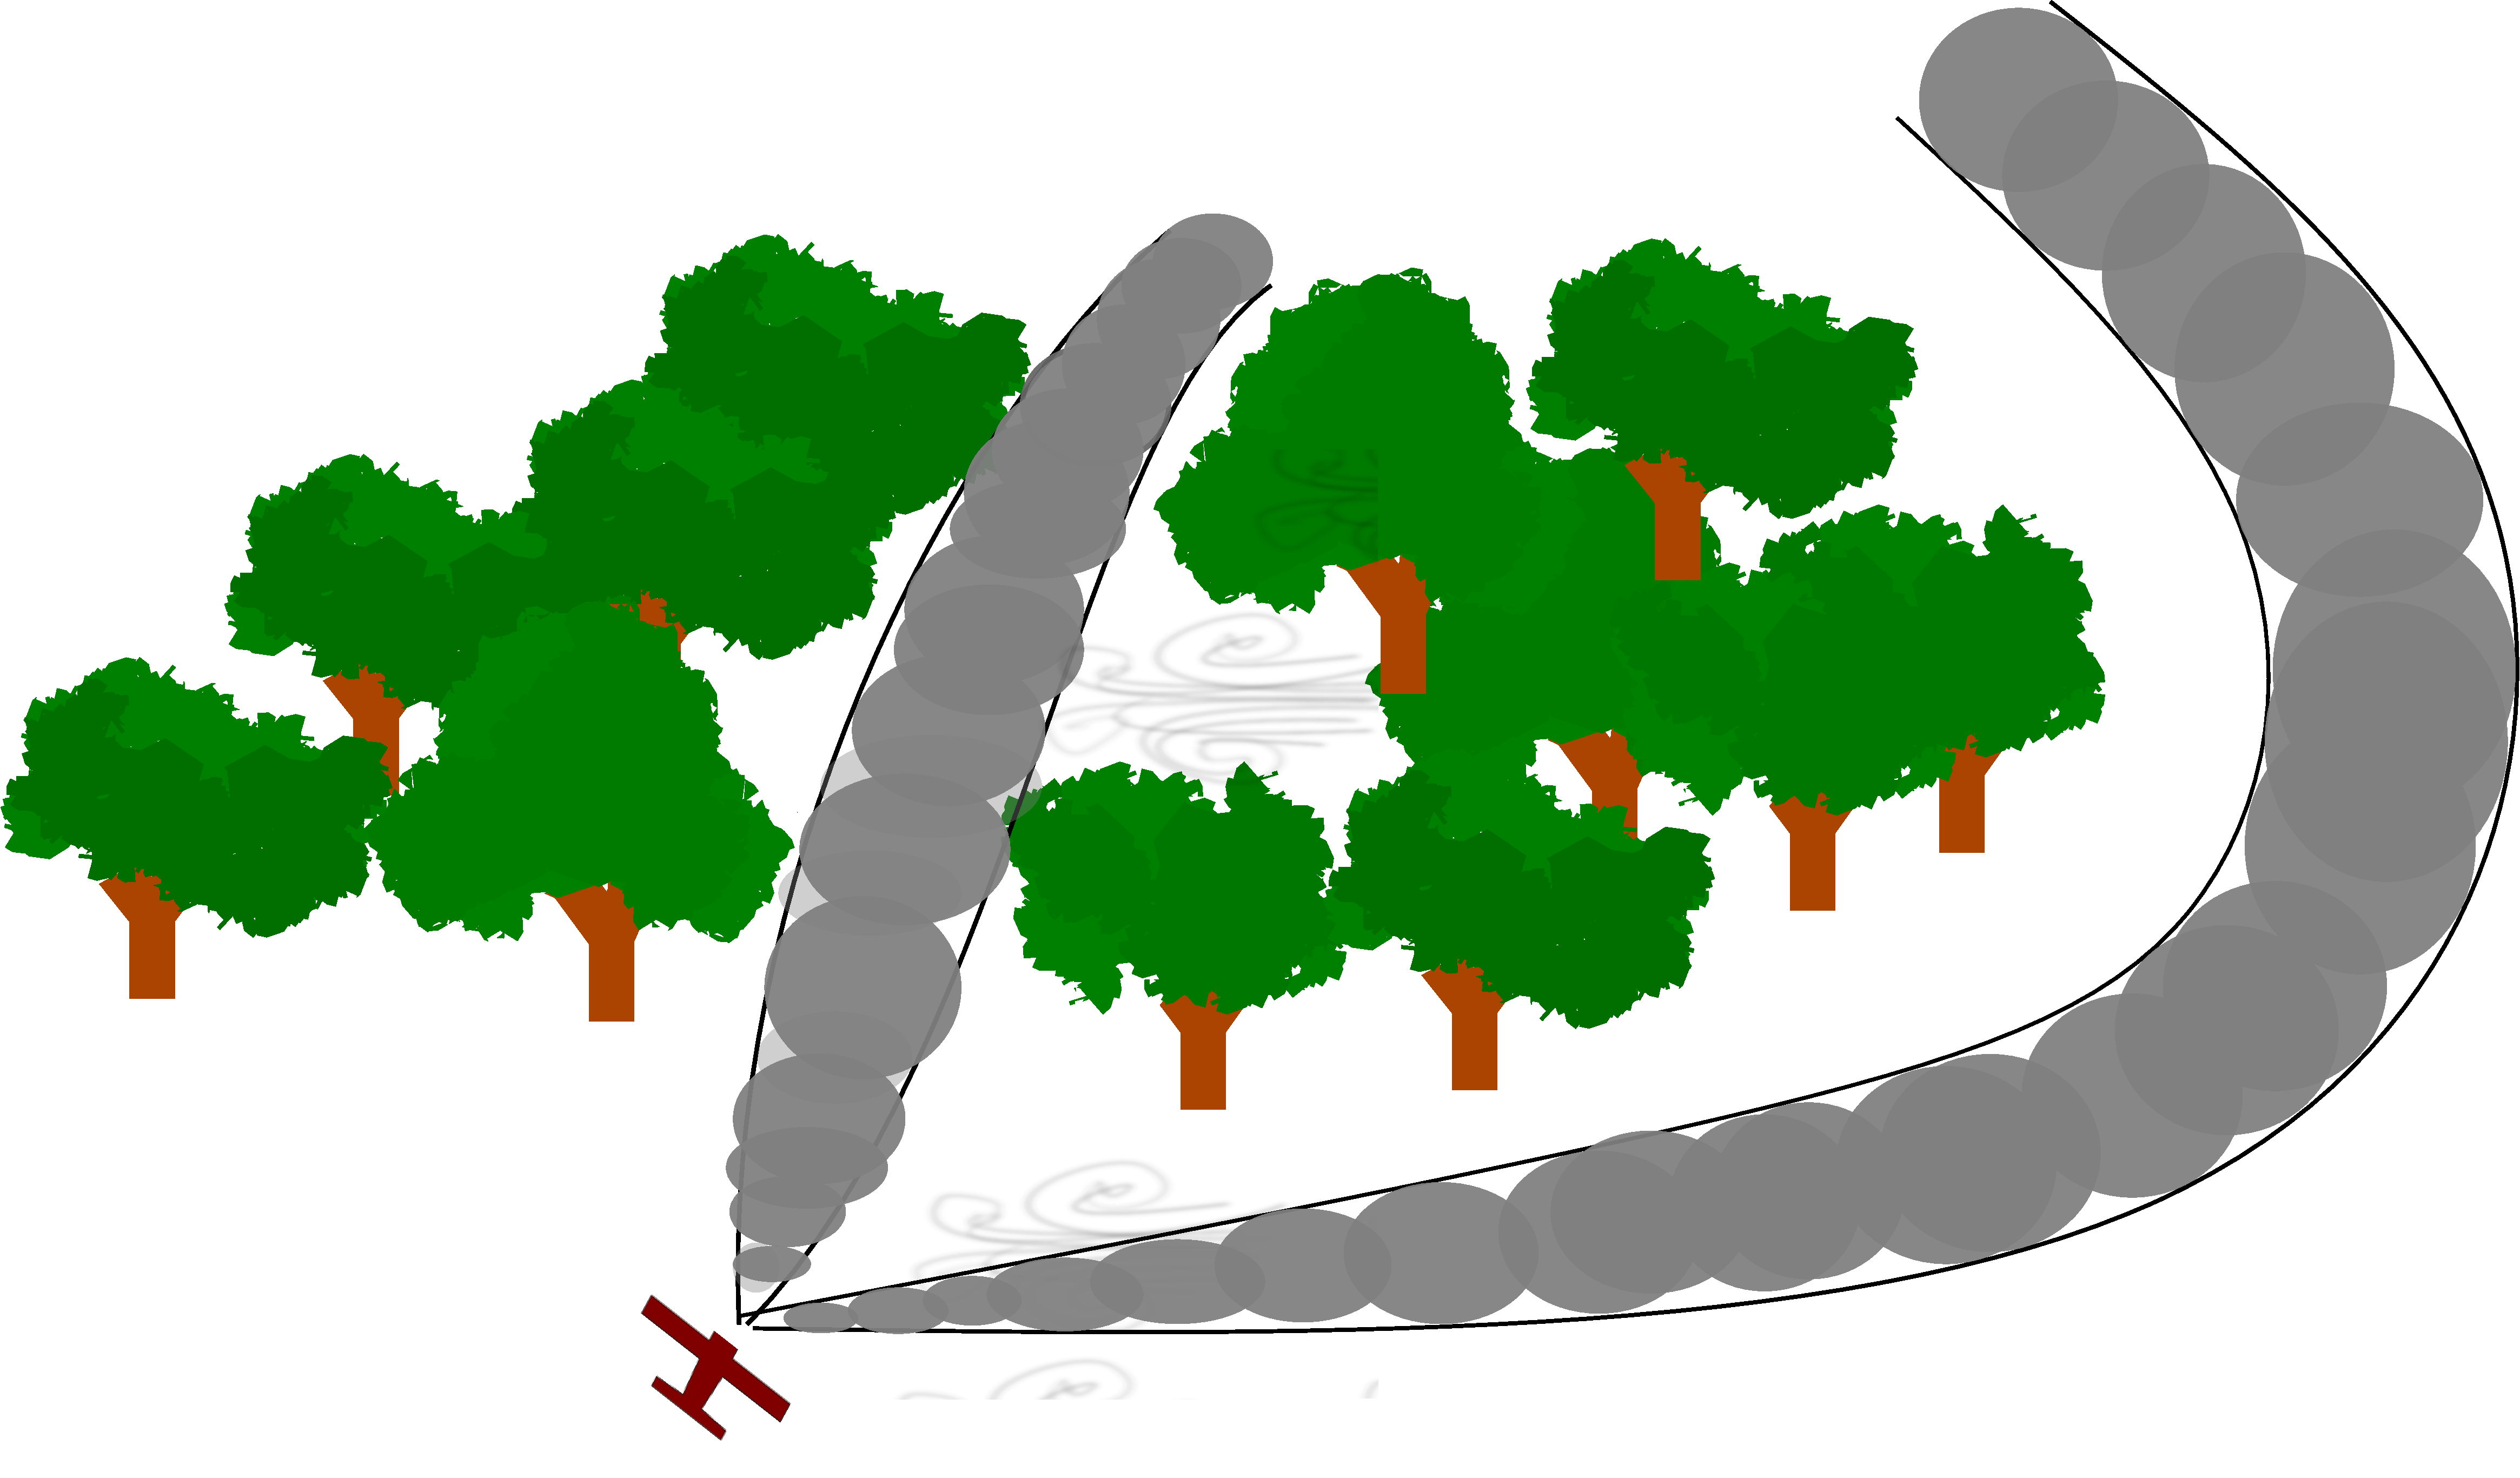
\includegraphics[width=.8\textwidth]{figures/experiments/aggressive-maneuver}
  \caption{A planner that is guaranteed to not collide might as well go straight
    through the opening in the forest, instead of the long way around an
    obstacle.}
  \label{fig:aggressive-maneuver}
\end{figure}

In general planning is harder for a nonlinear and non-holonomic vehicle, such as
the unicycle model employed in this thesis. Especially when uncertainty is added
to the model. In this case a lot of planners simply choose to ignore these error
sources and apply heuristics such as maximizing the distance to the obstacles in
the environment. However, this adds the disadvantage that the plans can become
overly conservative. Explicitly handling the uncertainties in the planning stage
enables the planner to employ more aggressive maneuvers, such as flying through
two trees close together, as opposed to flying around the entire grove. Flying
straight through is an acceptable maneuver for a planner that has guarantees on
the whereabouts of the dynamical system, and hence is not afraid to go close to
an obstacle. This confidence in planning is enabled by the calculation of
\textit{robust motion primitives} through the \ac{SOS} framework developed in
\cref{sec:funnels}. An example of this can be seen in
\cref{fig:aggressive-maneuver}.


As it currently stands the current implementation of the algorithm handles
uncertainty only in the position of the dynamical system, but can be easily
extended to handle uncertainty in input and speed as well by employing a
different dynamical model. Handling uncertainties in the environment is
currently not possible with the current approach. The algorithm is built up
through two main parts.

\subparagraph{} One is the calculation of \textit{robust motion primitives},
which allows the global motion planner (a regular \ac{RRT} algorithm) to remain
completely oblivious to these difficulties, and hence act as though there were
no uncertainties during the planning stage. This means that a lot of the
difficulty of planning is handled during the off-line phase of generating the
robust motion primitives themselves. The advent of \ac{SOS} programming enables
a numerical search for a Lyapunov function to verify the convergence of the
nonlinear feedback system. The one-level subset of the Lyapunov function is then
used as the reachable set of the dynamical system. Adding uncertainty to the
verification is simply the addition of a couple of extra constraints to the
\ac{SOS} program definition. Through formulating the search for a
\textit{Lyapunov function} for the system as a \ac{SOS} program, the
trajectories are extended to so called `funnels', which incorporate all the
states the system can be in during a given time frame -- even in the face of
uncertainties. In the literature this is referred to as a \textit{finite time
  reachable set}, meaning that if the calculations are correct, it contains all
the states that the system can evolve to in a given time frame from a set of
initial conditions and a bounded uncertainty term.


\subparagraph{} Second the aforementioned funnels are then employed as
\textit{motion primitives} for the global \ac{RRT} motion planning algorithm.
This means that they all encode a discrete action. For the dynamical system in
this thesis, which is a simple unicycle model, this means that the motion
primitives can be a simple `turn-left', `turn-right', or `go-straight' motion --
still a basis set for the planner should contain a richer collection of
primitives. Thus by stacking one motion primitive after the other, one is able
to create a plan, and hence build one long motion primitive through the
overarching environment. With the motion primitives being robust to uncertainty,
these plans are in theory guaranteed to be collision-free. The reason the theory
employed here does not necessarily apply to the real world is that most noise is
not bounded in the real world, and hence assumptions made may not be correct.


The \ac{RRT} algorithm can handle large state spaces and differential
constraints. However, it is not able to directly reason about uncertainty and
feedback during the planning stage. It is therefore that this thesis seeks to
combine the \ac{SOS} programming framework to generate robust motion primitives
for the \ac{RRT} algorithm which will use these primitives during the planning
stage, and hence can act like a normal \ac{RRT} algorithm, yet handle all the
difficulties of uncertainty and feedback at the same time, as this is all
contained in the motion primitives employed as branches in the planning tree.

\begin{figure}
  \centering
  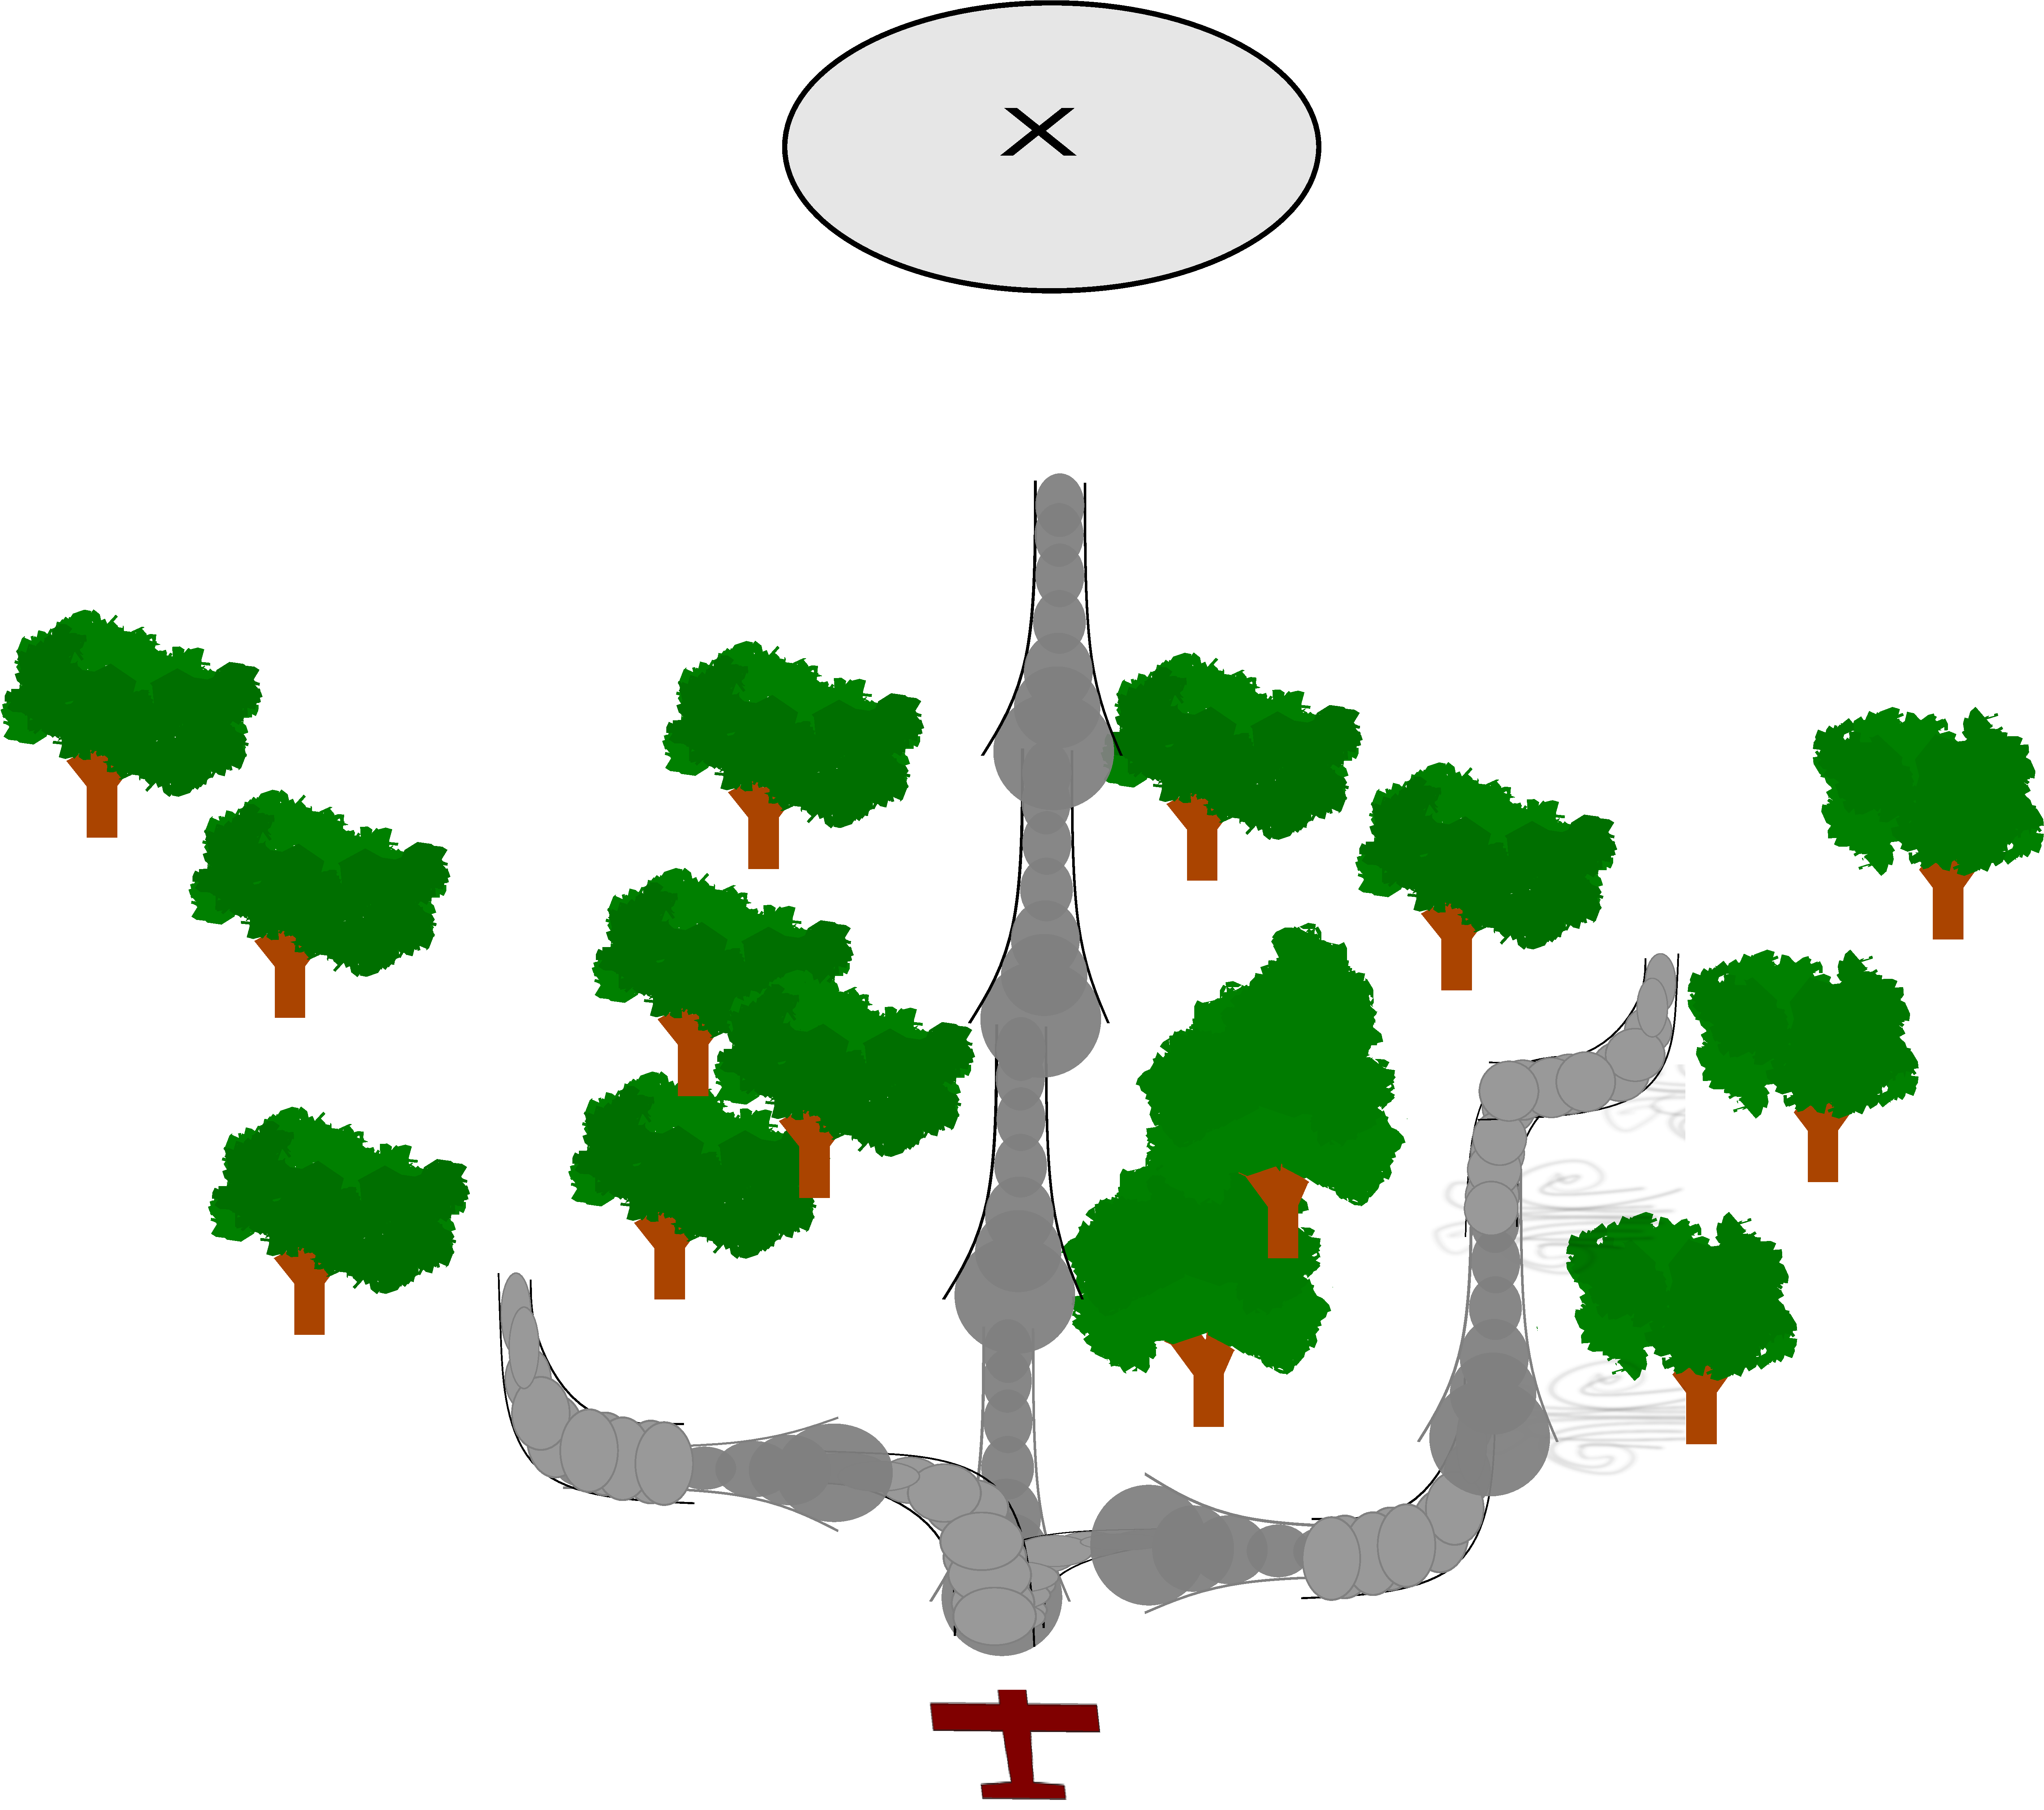
\includegraphics[scale=.1]{figures/experiments/experiment-airplane-strip}
  \caption{A cartoon of the experiment setup, showing how the \rrtfunnel{}
    algorithm builds a tree of funnels to find a safe path through a strip of
    forest.}
  \label{fig:experiments-cartoon}
\end{figure}

\paragraph{Experiments}
This theoretical robustness guarantee is later put to the test in simulated
experimental runs through a strip of forest of some density meant to make
planning difficult, along with a cross-wind given to the system as noise. A
cartoon of the experiment environment can be seen in
\cref{fig:experiments-cartoon}. Hence the airplane is constantly faced with a
positional offset, and is forced to deal with this as best as it is able to
during execution of the plan. As is shown, the robustness guarantees provided by
the Lyapunov functions found through the \ac{SOS} programs formulated, do
provide safe traversal through the environment, as opposed to a planner which
does not.

